% !TEX root = paper.tex

\section{Performance Results} \label{sec:experiments}

% !TEX root = experiments.tex

% macros for plotting
\newcommand{\datafile}{}
\newcommand{\alg}{}
\newcommand{\numiterations}{30}
\newcommand{\minvalue}{1}

% toggles whether or not to plot naive results (if not, the rows of the data file also need to be commented out)
\newif\ifnaive
% toggles ksweep vs scaling plot
\newif\ifksweep
% toggles legend
\newif\iflegend
% toggles y axis label
\newif\ifylabel
% toggles wider plot area
\newif\ifwider
% toggles including liavas results
\newif\ifliavas


\newcommand{\setcolors}{
\pgfplotsset{cycle list={
	red, fill=red \\ 
	blue, fill=blue \\ 
	green, fill=green \\ 
	red, pattern=crosshatch, pattern color=red \\
	green, pattern=crosshatch, pattern color=green \\
	blue, pattern=crosshatch, pattern color=blue \\
}};
}

% set options for grouped bar plot
\newcommand{\breakdownplotoptions}{
	ybar stacked,
	reverse legend,
	bar width=8pt,
	width=9cm, height=3.85cm,
	ylabel={Time (s)}, 
	y label style={yshift=-.5cm},
	ymin=0,
	symbolic x coords={D1,N1,D16,N16,D81,N81,D256,N256},
	xtick=data,
	legend style={at={(0.5,1.3)},anchor=north},
	legend columns=-1,
	reverse legend
}

% stacked bar plot command
\newcommand{\breakdownplot}{
\begin{axis}[\breakdownplotoptions]
	\setcolors
	\addplot table[x=alg-p, y expr=(\thisrow{mttkrp}/(\minvalue*\numiterations))] {\datafile};
	\addplot table[x=alg-p, y expr=(\thisrow{krp}/(\minvalue*\numiterations))] {\datafile};
	\addplot table[x=alg-p, y expr=((\thisrow{allgather}+\thisrow{reducescatter})/(\minvalue*\numiterations))] {\datafile};
	\addplot table[x=alg-p, y expr=((\thisrow{nnls}+\thisrow{gram}+\thisrow{allreduce})/(\minvalue*\numiterations))] {\datafile};
	\addplot table[x=alg-p, y expr=((\thisrow{err_compute}+\thisrow{err_communication})/(\minvalue*\numiterations))] {\datafile};
	\legend{MTTKRP,KRP,Factor Comm,NLS,Error};
\end{axis}
}

% labels for bar groups (manually positioned)
\newcommand{\labels}{
%\node [align=center,text width=3cm] at (1.25cm, -.95cm)   {\ifksweep 10 \else 16 \fi};
%\node [align=center,text width=3cm] at (3cm, -0.95cm)   {\ifksweep 20 \else 96 \fi};
%\node [align=center,text width=3cm] at (4.6cm, -0.95cm)   {\ifksweep 30 \else 384 \fi};
%\node [align=center,text width=3cm] at (6.3cm, -0.95cm) {\ifksweep 40 \else 864 \fi};
%\node [align=center,text width=3cm] at (8.15cm, -0.95cm) {\ifksweep 50 \else 1536 \fi};
\node [align=center,text width=3cm] at (1cm, -1.15cm)   {\ifksweep 10 \else 1 \fi};
\node [align=center,text width=3cm] at (2.4cm, -1.15cm)   {\ifksweep 20 \else 16 \fi};
\node [align=center,text width=3cm] at (3.7cm, -1.15cm)   {\ifksweep 30 \else 81 \fi};
\node [align=center,text width=3cm] at (5.1cm, -1.15cm) {\ifksweep 40 \else 256 \fi};
}

% allows for filtering rows from dat file
\pgfplotsset{
    discard if not/.style 2 args={
        x filter/.append code={
            \edef\tempa{\thisrow{#1}}
            \edef\tempb{#2}
            \ifx\tempa\tempb
            \else
                \def\pgfmathresult{inf}
            \fi
        }
    }
}

% set options for strongscaling plot
\newcommand{\strongscalingplotoptions}{
		log basis y={2},
		log basis x={2},
		\ifliavas
			xlabel=Cores,
		\else
			xlabel=Nodes,
		\fi
		ylabel=Time (s),
		y tick label style={
	        /pgf/number format/.cd,
            	precision=4,
		},
	legend style={draw=none, cells={align=left}, nodes={scale=0.7}}
}

% plot time over p, filtering rows out appropriately
\newcommand{\strongscalingplot}{
\begin{loglogaxis}[\strongscalingplotoptions]
	%\addplot+ [discard if not={alg}{N},thick,mark options={solid},mark=square*] table [x={p}, y={totaltime}] {\datafile};
	\ifliavas
		\addplot+ [discard if not={alg}{DF},thick,mark options={solid},mark=square*] table [x={p}, y expr=(\thisrow{total}/(\minvalue*\numiterations))] {\datafile};
		\addplot+ [discard if not={alg}{NF},thick,mark options={solid},mark=square*] table [x={p}, y expr=(\thisrow{total}/(\minvalue*\numiterations))] {\datafile};
	\else
		\addplot+ [discard if not={alg}{D},thick,mark options={solid},mark=triangle*] table [x={p}, y expr=(\thisrow{total}/(\minvalue*\numiterations))] {\datafile};
		\addplot+ [discard if not={alg}{N},thick,mark options={solid},mark=square*] table [x={p}, y expr=(\thisrow{total}/(\minvalue*\numiterations))] {\datafile};
	\fi
	\ifliavas
		\addplot+ [discard if not={alg}{L},thick,mark options={solid}] table [x={p}, y expr=(\thisrow{total}/(\minvalue*\numiterations))] {\datafile};
		\legend{DimTree,NoDimTree,NbAO-NTF \cite{LK+17b}}
	\else
		\legend{DimTree,NoDimTree,FlatDimTree,FlatNoDimTree};
	\fi
\end{loglogaxis}
}



\subsection{Datasets}

\GB{This section is out of date...}

\subsubsection{Hyperspectral Images (HSI)}
For comparison with previous work \cite{LK+17b}, we consider the same 3D hyperspectral imaging dataset called ``Souto\_wood\_pile'' \cite{FAN16}. 
NNCP is often used on HSI data sets for classification and blind source separation of materials with differing spectral signatures.
The hyperspectral datacube has dimensions $1024 \times 1344 \times 33$ and represents a set of 33 grayscale images of size 1344 $\times$ 1024 pixels sampled at wavelengths 400, 410, $\dots$, 720 nm, with each pixel value representing spectral radiance in $W m^{-2} sr^{-1} nm^{-1}$. 
We also consider the Nogueir\'{o} scene dataset, which is a sequence of 9 time-lapse HSI images of the same scene acquired at about 1-hour intervals.
In each scene, hyperspectral images were acquired at about 1-hour intervals. 
Each Nogueir\'{o} scene HSI image has the same properties as the Souto\_wood\_pile data set, so the corresponding tensor has dimensions $1024 \times 1344 \times 33 \times 9$. 

\subsubsection{Dynamic Functional Connectivity (dFC)}
We also consider dynamic functional connectivity datasets that are generated from fMRI images of human brains.
Given a 4D fMRI data set of voxel measurements across multiple timesteps, voxels containing brain data are partitioned into a set of regions of interest (specified using domain-specific knowledge), and a single time-series signal is aggregated for each region of interest.
Then, an instantaneous correlation is computed for each time point and pair of regions, and this process is repeated for a number of subjects.
Computing a CP decomposition of this data helps to discover patterns of brain connectivity among different regions and also differentiate among individuals.
For our representative dFC data set, we consider 246 brain regions, which yields 30{,}012 unique pairs of regions, 1200 times steps, and 500 subjects, or a tensor of dimension $30{,}012\times 1200 \times 500$ \cite{VEU+12,THBGW17}.

\subsubsection{Synthetic}
Our synthetic data sets are constructed from a CP model with an exact low rank with no added noise.
In this case we can confirm that the residual error of our algorithm with a random start converges to zero.
For the purposes of benchmarking, we run a fixed number of iterations of the BCD algorithm rather than using a convergence check.

%For the synthetic datasets, our open source code supports (a) low-rank tensor (b) uniform random and (c) positive shifted normal distribution of $\mathfrak{N}(3,1)$ -- that is change the mean such that all the random numbers are positive. We considered three different synthetic matrices for different cases. For baseline comparison with Liavas \cite{LK+17b}, we considered a three mode 
%uniform of size 1024x1024x1024 on processor grids $2^k \times 2^k \times 2^k$ for $k \in {0,1,2,3}$. We used the uniform five 
%mode synthetic tensor with dimension $64\times 64\times 64\times 64\times 64$ on processor grids 
%$1\times1\times1\times1\times1$, $2\times1\times1\times1\times1$, $\dots$, $2\times2\times2\times2\times2$ for strong scaling 
%experiments.  In the case of weak scaling of four mode synthetic tensors with (D) and without (N) the use of dimension trees.  The 
%tensor and processor grid dimensions are $128k\times 128k\times 128k\times 128k$ and $k\times k\times k\times k$ for $k\in\{1,2,3,4\}$. In all the cases the dimensions were considered such that synthetic tensors can be accommodated even on single node with 64GB for scale up plots. 

\subsection{Machine Details}

\GB{This section is out of date...}

The entire experimentation was performed on Eos, a supercomputer at the Oak Ridge Leadership Computing Facility. 
Eos is a 736-node Cray XC30 cluster of Intel Xeon E5-2670 processors with a total of 47.104TB of memory. 
Its compute nodes are organized in blades where each blade contains 4 nodes, and every node has 2 sockets with 8 physical cores and 64GB memory. 
The machine support Intel's hyper-threading (HT), but we restricted it because HT offers minimal improvement for BLAS and LAPACK operations. 
In total, the Eos compute partition contains 11,776 traditional processor cores and our experiments used up to 4,096 cores (35\% of the machine). 

Our objective of the implementation is using open source software as much as possible 
to promote reproducibility and reuse of our code.
%Unlike Liavas \cite{LK+17b} that uses Eigen matrix library \cite{eigenweb}, 
We use Armadillo \cite{sanderson2010} for matrix representation
and operations.  
In Armadillo, the elements of the dense matrix are stored in column major order.
For dense BLAS and LAPACK operations, we linked Armadillo with the default LAPACK/BLAS wrappers from Cray. 
For compiler, we use GNU C++ Compiler (g++ (GCC) 6.3.0) and MPI library is from Cray.  We could also 
compile and run the code in Rhea the commodity cluster from OLCF with entire open source libraries such as OpenBLAS and OpenMPI. 

\subsection{Microbenchmarks with Synthetic Data}

\subsubsection{Comparison across Algorithms}

\begin{itemize}
	\item MU and CP-ALS clearly cheapest, should scale like $k^2$
	\item Nesterov most expensive, due to inner iterations
	\item HALS, AO-ADMM, Nesterov all involve communication during ``LUC"
\end{itemize}

%%%%%%%%%%%%%%%%%
%LUC Running Time Comparison
%%%%%%%%%%%%%%%%%

\begin{figure}
\subfloat[Synthetic Low Rank \label{fig:luclr81}]{
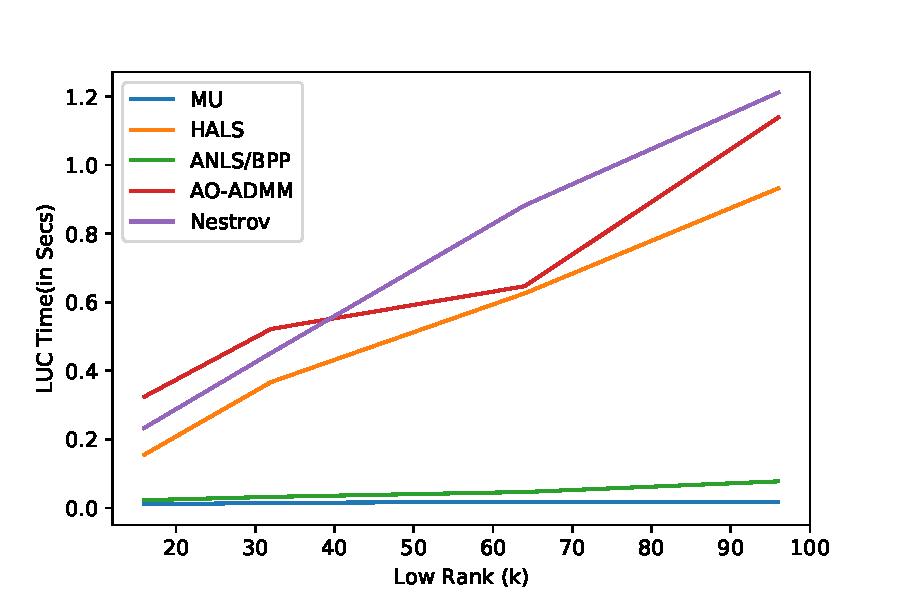
\includegraphics[width=0.45\textwidth, height=2in]{data/plots/luclr81.pdf}
}
\subfloat[Tiny Imagenet \label{fig:lucrw}]{
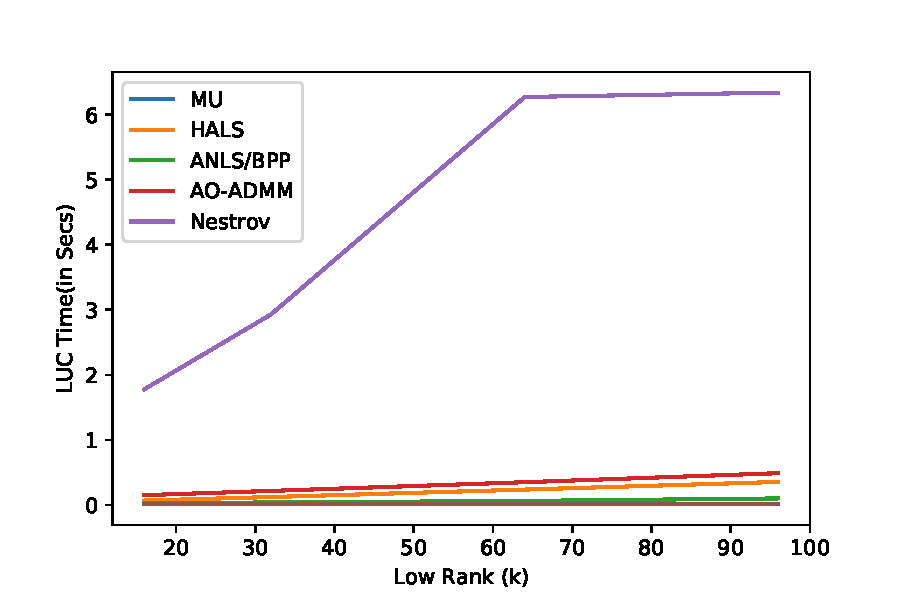
\includegraphics[width=0.45\textwidth, height=2in]{data/plots/lucrw64.pdf}
}
\caption{LUC comparison of \MU, \HALS, \BPP, \ADMM, \Nestrov\ on 4D Synthetic Low Rank Tensor of size $384 \times 384 \times 384 \times 384$ on 81 Titan nodes as 3x3x3x3 Processor Grid on CPU and Realworld TinyImagenet Dataset on 64 Titan nodes as 2x4x2x4 processor grid}
\label{fig:luccomp}
\end{figure}

\subsubsection{Comparison across Processor Grids}

%%%%%%%%%%%%%%%%%
%Configuration Sweep
%%%%%%%%%%%%%%%%%
\begin{figure}
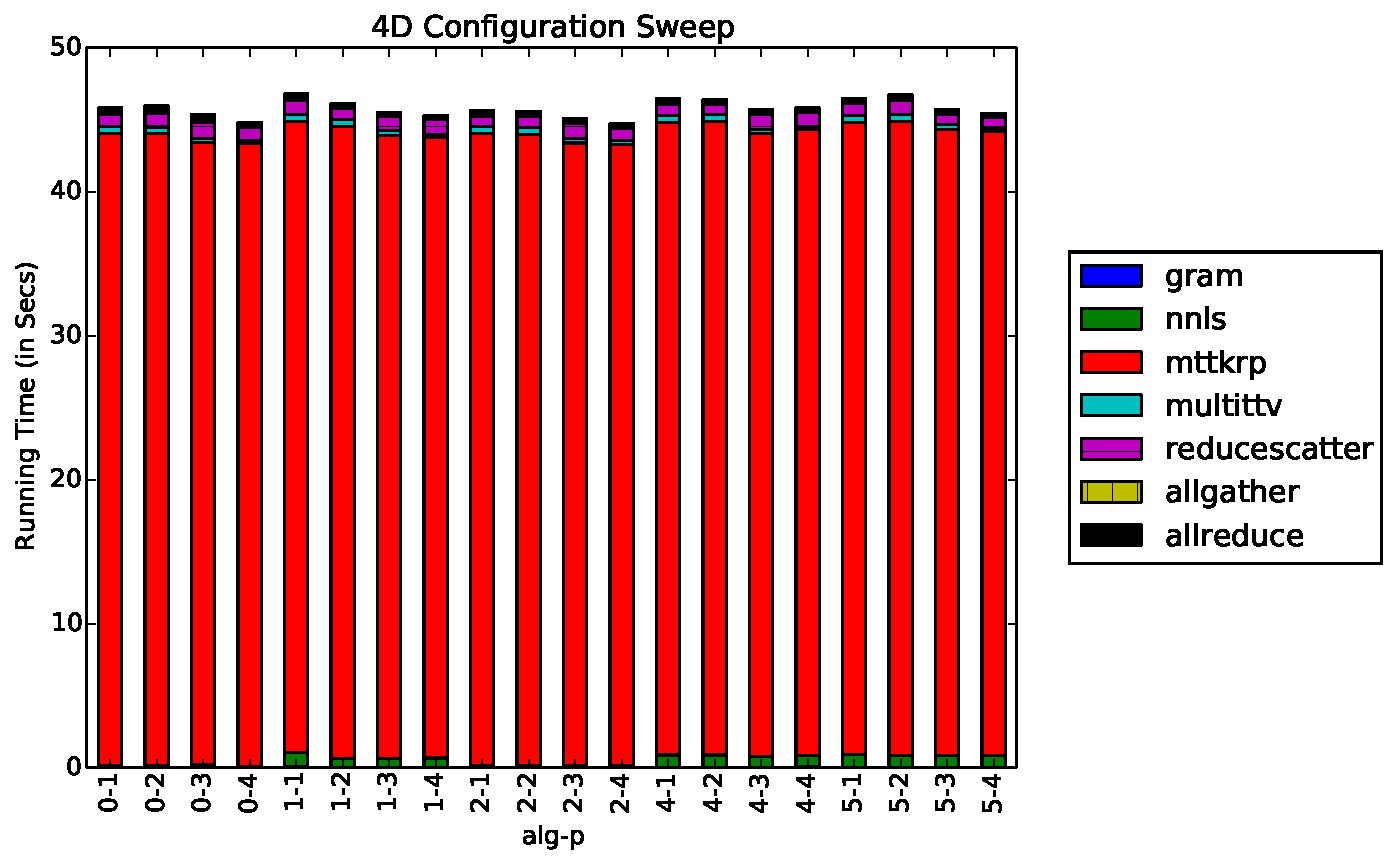
\includegraphics[width=\textwidth, height=2.5in]{data/plots/confsweep4d.pdf}
\caption{Processor Grid sweep of a $384 \times 384 \times 384 \times 384$ synthetic low rank tensor on 81 nodes in Titan as 81x1x1x1, 27x3x1x1, 9x3x3x3, 3x3x3x3 grids represented as p=1,2,3,4 respectively. The algorithms alg=0,1,2,4,5 are \MU, \HALS, \BPP, \ADMM, \Nestrov\ respectively.}
\label{fig:confsweep4D}
\end{figure}

\subsection{Scaling Studies with Synthetic Data}

\subsubsection{Weak Scaling}

%%%%%%%%%%%%%%%%%
%Weak Scaling Synthetic Low Rank
%%%%%%%%%%%%%%%%%
\begin{figure}
\subfloat[Synthetic 3D Low Rank \label{fig:wksca3d}]{
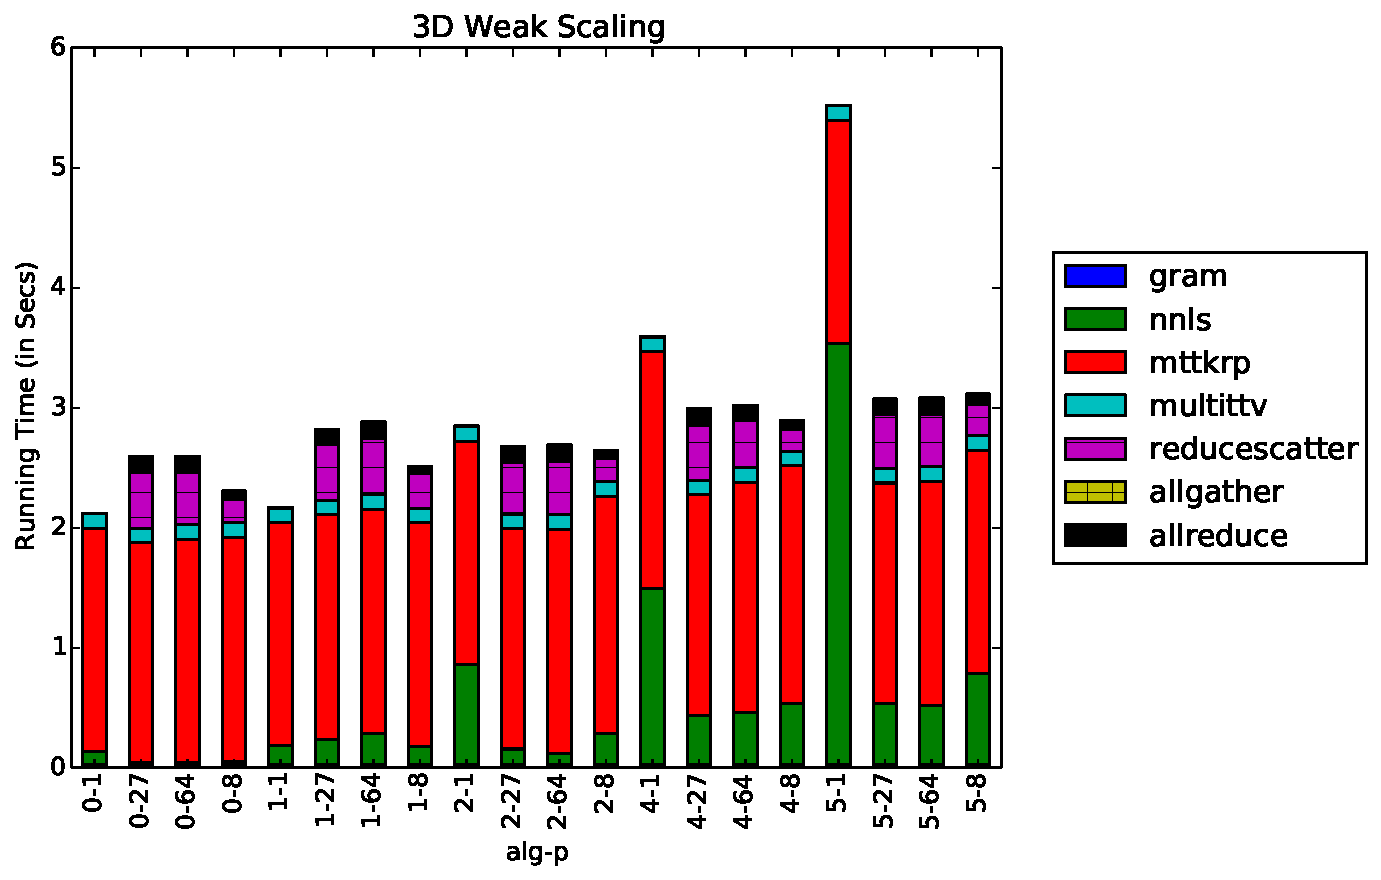
\includegraphics[width=\textwidth, height=3in]{data/plots/wksca3d.pdf}
}\\
\subfloat[Synthetic 4D Low Rank \label{fig:wksca4d}]{
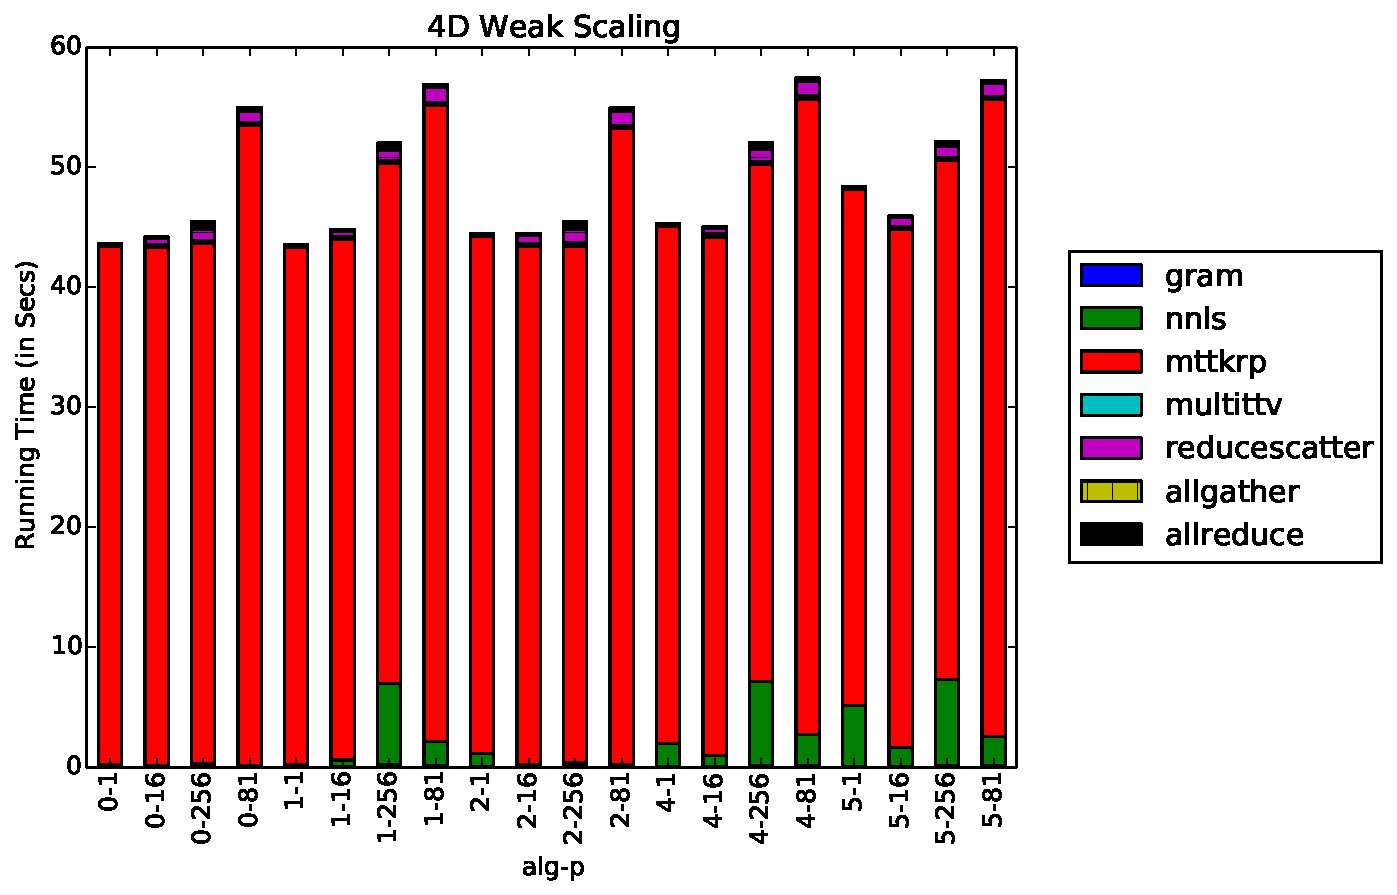
\includegraphics[width=\textwidth, height=3in]{data/plots/wksca4d.pdf}
}
\caption {Weak Scaling on Synthetic 3D and 4D low rank tensors. For 3D, the input tensor is of size 128x128x128, 256x256x256, 378x378x378 and 512x512x512 on 1, 8, 27 and 64 Titan Nodes. The 4D tensors were of size 128, 256, 405, 512 for each mode on 1, 16, 81 and 256 Titan nodes.  The algorithms alg=0,1,2,4,5 are \MU, \HALS, \BPP, \ADMM, \Nestrov\ respectively.}
\label{fig:synweakscaling}
\end{figure}

\subsubsection{Strong Scaling}

%%%%%%%%%%%%%%%%%
%Strong Scaling Synthetic Low Rank
%%%%%%%%%%%%%%%%%
\begin{figure}
\subfloat[Synthetic 3D Low Rank \label{fig:strsca3d}]{
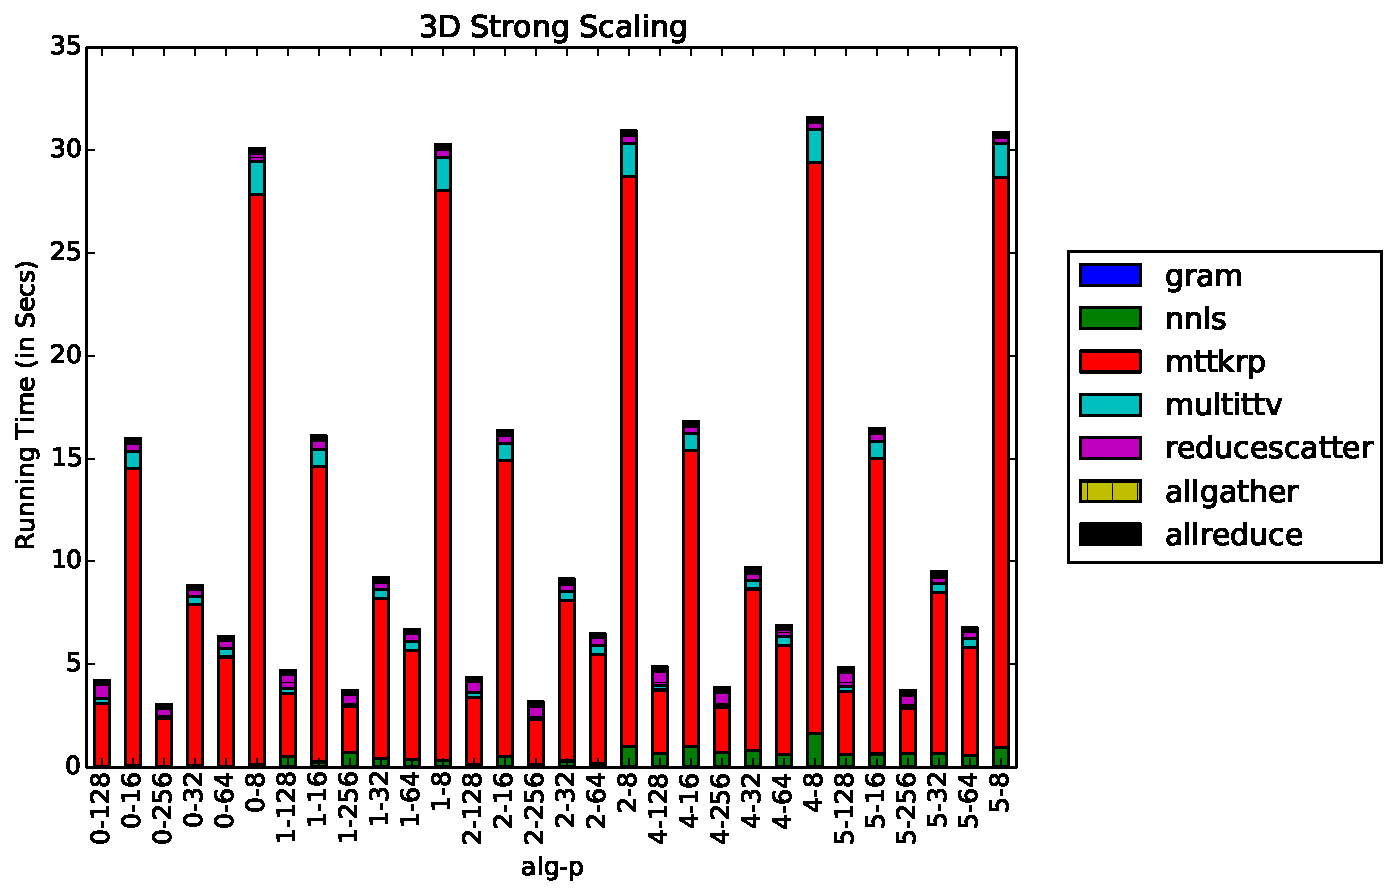
\includegraphics[width=\textwidth, height=3in]{data/plots/strsca3d.pdf}
}\\
\subfloat[Synthetic 4D Low Rank \label{fig:strsca4d}]{
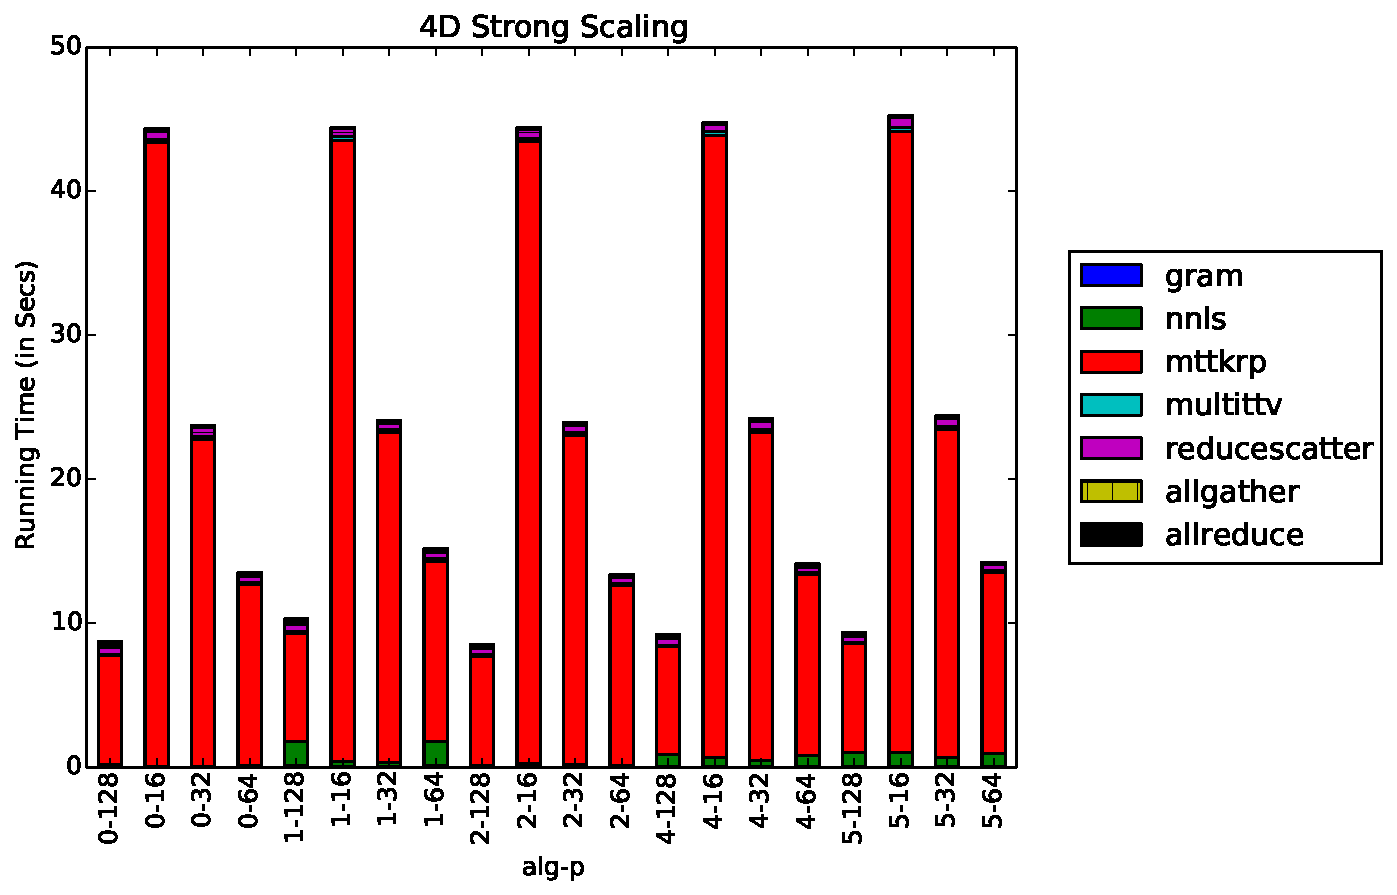
\includegraphics[width=\textwidth, height=3in]{data/plots/strsca4d.pdf}
}
\caption {Strong Scaling on Synthetic 3D and 4D low rank tensors. For 3D, the input tensor is of size 1024x1024x1024 and 256x256x256x256 for 4D on 8,16, 32, 64 and 128 nodes in Titan. The algorithms alg=0,1,2,4,5 are \MU, \HALS, \BPP, \ADMM, \Nestrov\ respectively.}
\label{fig:synstrongscaling}
\end{figure}

\GB{Everything after this point is still disorganized...}

\subsection{Varying Approximation Rank}

One of the challenges of the CP (and NNCP) decomposition in practice is the choice of decomposition rank.
The most common technique is to compute multiple CP decompositions for various ranks.
As the rank $R$ increases, the approximation error  $\|\TA - \T{M}\|$ decreases with the better approximation power of more parameters. 
However, the benefit of increasing $R$ eventually diminishes if the data can be well approximated with a CP model.
%that an increase in $R$ in lower values, say from 5 to 10, will have significant improvement in relative error over increase in higher 
%values, like 100 to 105. 
%Hence, it is common practice in the community to sweep $k$, to obtain better approximation error within the 
%manageable computation. 
Towards this end, we experiment with various values of $R$ to observe the relative increase in running time for two real-world data sets. 

%%%%%%%%%%%%%%%%%
%Convergence Plot for Synthetic low rank
%%%%%%%%%%%%%%%%%

\begin{figure}
\subfloat[Low rank $k=64$ \label{fig:accuracylr81k64}]{
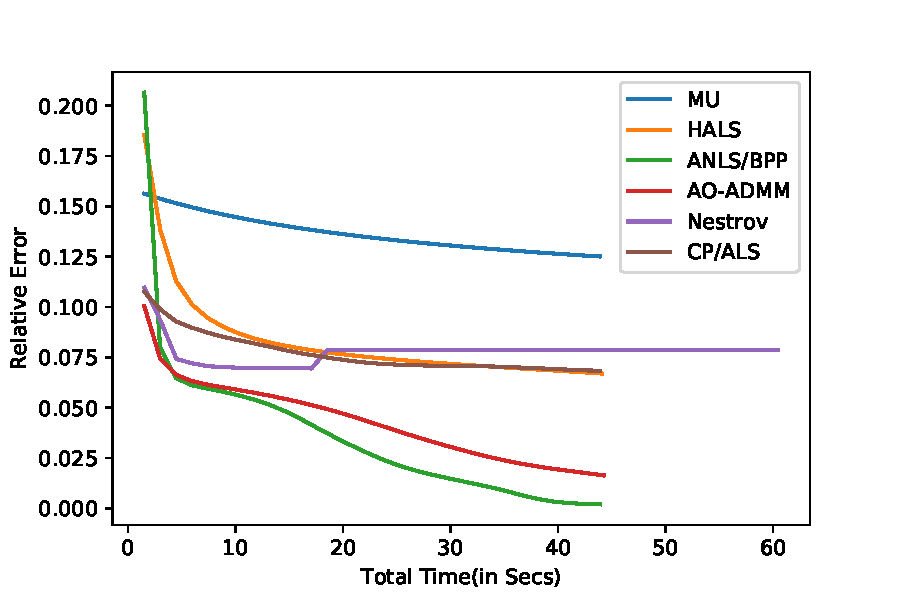
\includegraphics[width=0.45\textwidth, height=2in]{data/plots/accuracylr64.pdf}
}
\subfloat[Low rank $k=96$ \label{fig:accuracylr81k96}]{
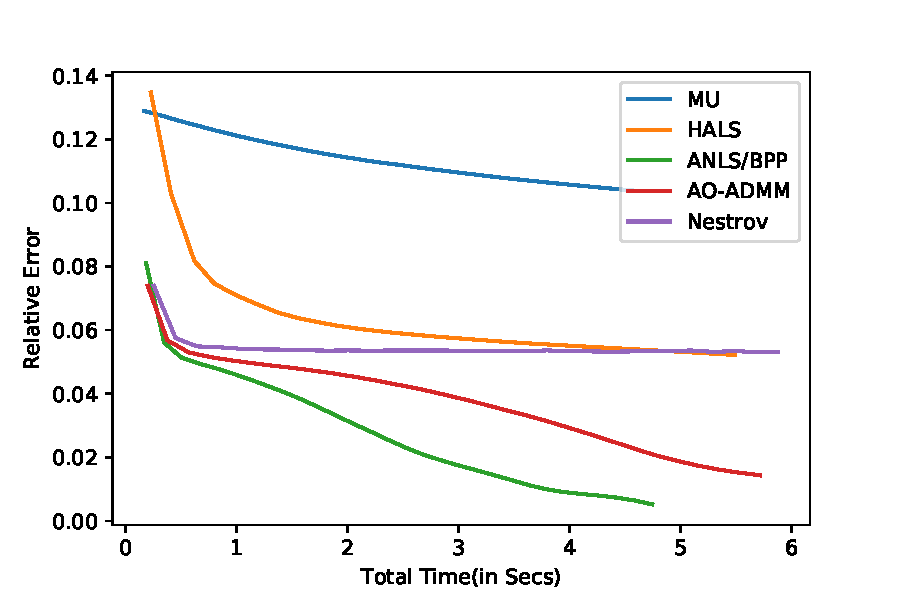
\includegraphics[width=0.45\textwidth, height=2in]{data/plots/accuracylr96.pdf}
}
\caption{Relative error comparison of \MU, \HALS, \BPP\, \ADMM, \Nestrov\ on 4D Synthetic Low Rank Tensor of size 384x384x384x384 on 81 Titan Nodes as 3x3x3x3 Processor Grid.}
\label{fig:convergencelowrank}
\end{figure}

%%%%%%%%%%%%%%%%%
%Convergence Plot for Realworld
%%%%%%%%%%%%%%%%%

\begin{figure}
	\subfloat[Low rank $k=64$ \label{fig:accuracyrwk64}]{
		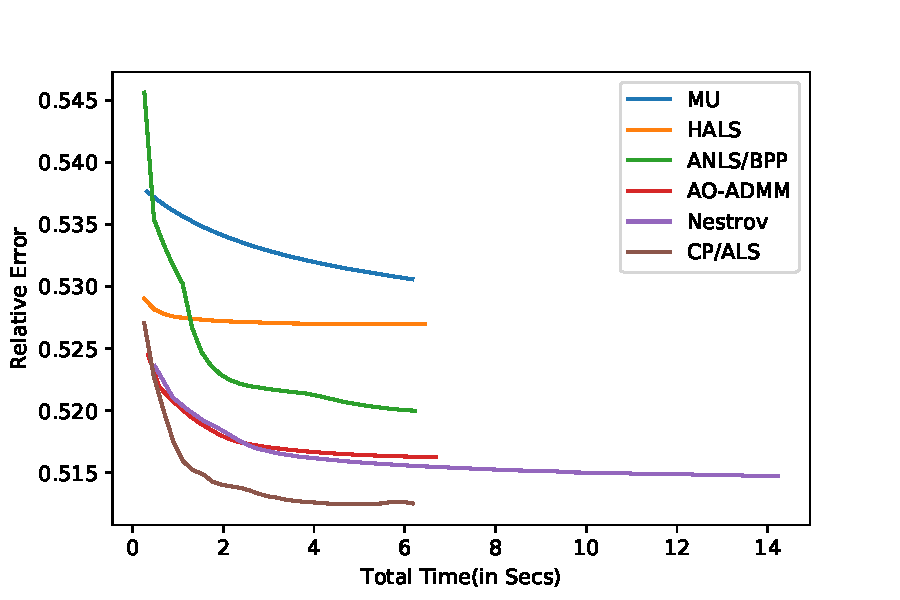
\includegraphics[width=0.45\textwidth, height=2in]{data/plots/accuracyrw64.pdf}
	}
	\subfloat[Low rank $k=96$ \label{fig:accuracyrwk96}]{
		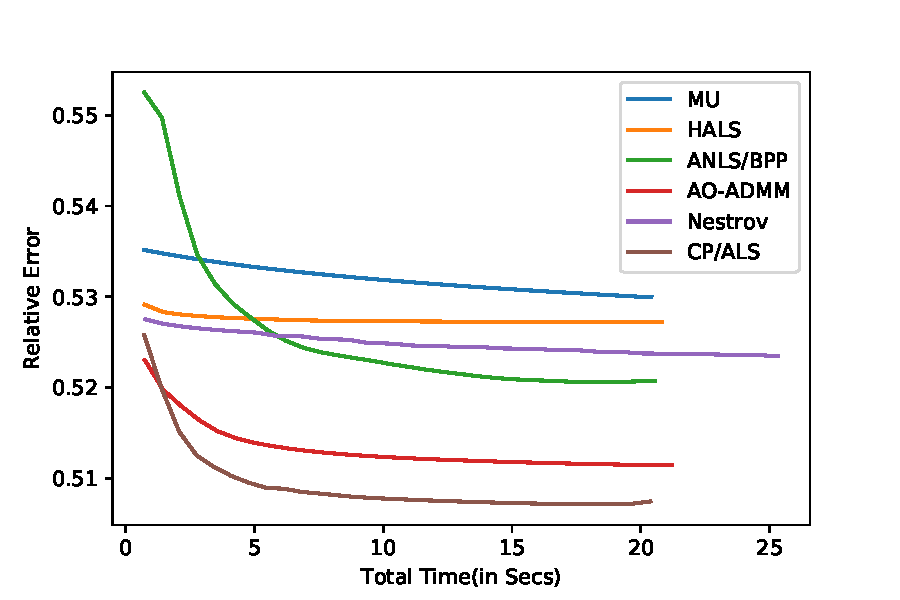
\includegraphics[width=0.45\textwidth, height=2in]{data/plots/accuracyrw96.pdf}
	}
	\caption{Relative error comparison of \MU, \HALS, \BPP\, \ADMM, \Nestrov\ on 4D Realworld Low Rank Tensor of size $200 \times 500 \times 64 \times 192$ on 64 Titan Nodes as $4\times4\times1\times4$ Processor Grid.}
	\label{fig:convergencerealworld}
\end{figure}


%%%%%%%%%%%%%%%%%
%CPU VS GPU on Synthetic Low Rank and Realworld
%%%%%%%%%%%%%%%%%

\begin{figure}

\subfloat[CPU \label{fig:cpulr81}]{
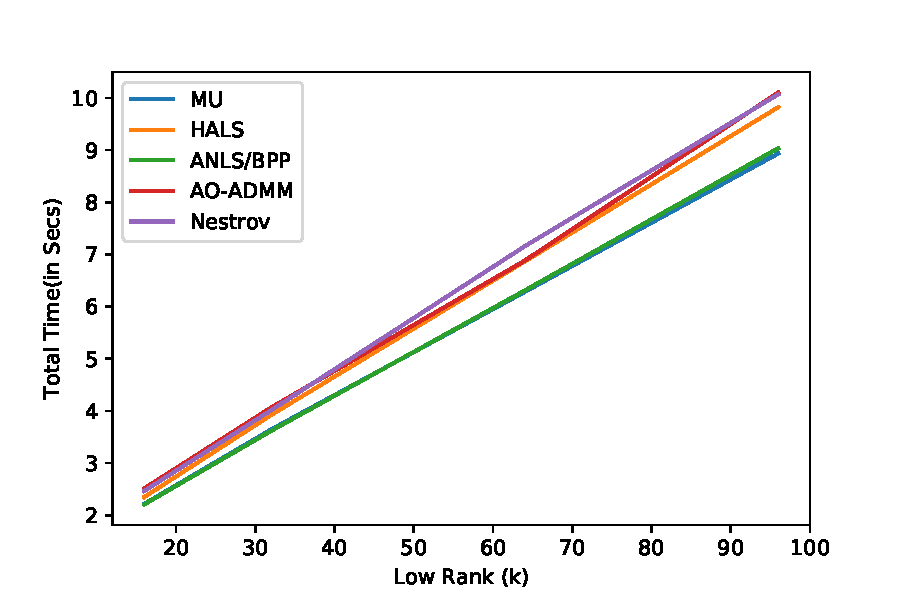
\includegraphics[width=0.45\textwidth, height=2in]{data/plots/cpuvsgpulr810.pdf}
}
\subfloat[GPU \label{fig:gpulr81}]{
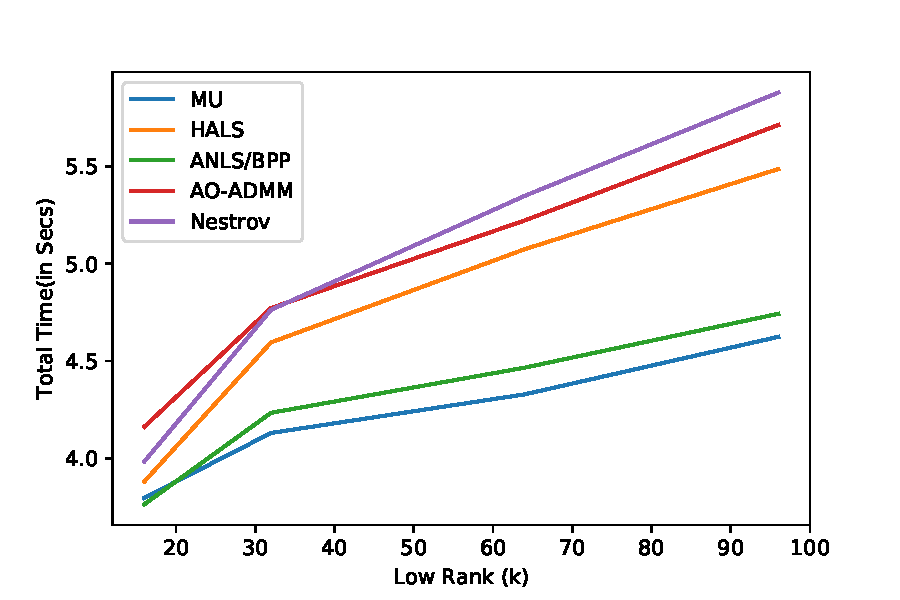
\includegraphics[width=0.45\textwidth, height=2in]{data/plots/cpuvsgpulr811.pdf}
}
\caption{Timing comparison of \MU, \HALS, \BPP\, \ADMM, \Nestrov\ on 4D Synthetic Low Rank Tensor of size 384x384x384x384 on 81 Titan Nodes as 3x3x3x3 Processor Grid on CPU and GPU.}
\label{fig:cpuvsgpulowrank}
\end{figure}



\subsection{Strong Scaling Time Breakdown}



%%%%%%%%%%%%%%%%%
%Strong Scaling Realworld Low Rank
%%%%%%%%%%%%%%%%%
\begin{figure}
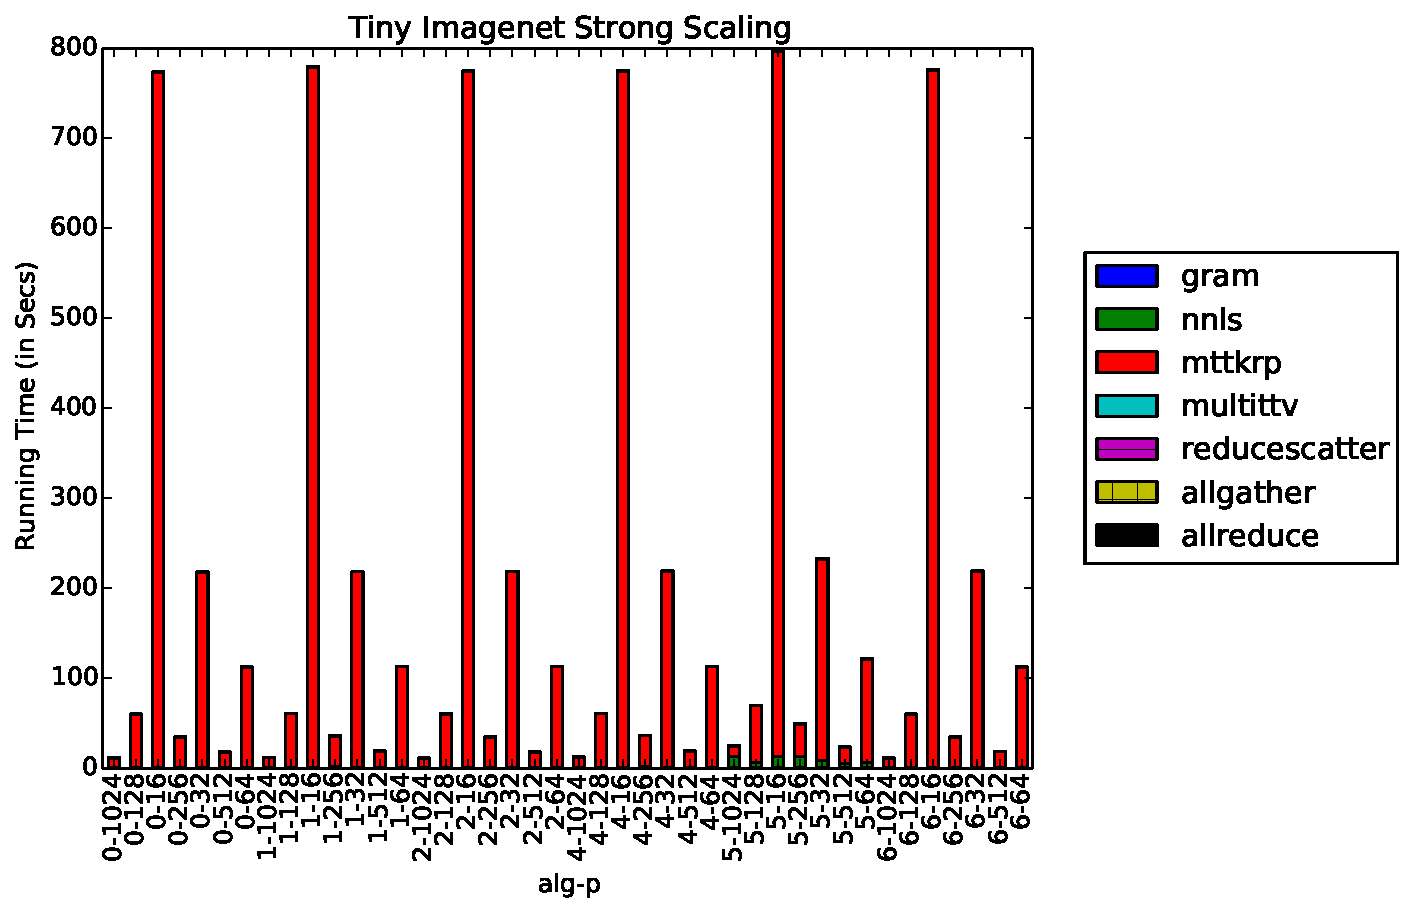
\includegraphics[width=\textwidth, height=3in]{data/plots/ssrw_tinyimagenet_breakdown.pdf}
\caption {Strong Scaling on Realworld Tiny Imagenet Dataset on 32, 64, 128, 256, 512 and 1024 nodes in Titan. The algorithms alg=0,1,2,4,5,6 are \MU, \HALS, \BPP, \ADMM, \Nestrov, \CPALS\ respectively.}
\label{fig:synstrongscaling}
\end{figure}

\subsection{Weak Scaling Time Breakdown}





\subsection{Varying Processor Grid}



%%%%%%%%%%%%%%%%%
%Mouse Data
%%%%%%%%%%%%%%%%%
\begin{figure}
	\subfloat[Low rank $k=64$ \label{fig:accuracyrwk64}]{
		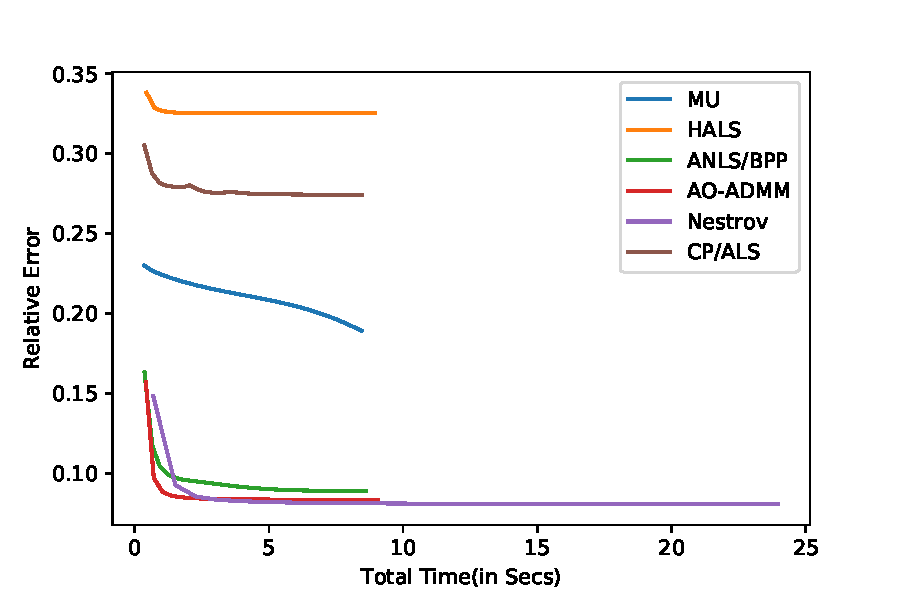
\includegraphics[width=0.45\textwidth, height=2in]{data/plots/accuracymouse64.pdf}
	}
	\subfloat[Low rank $k=96$ \label{fig:accuracyrwk96}]{
		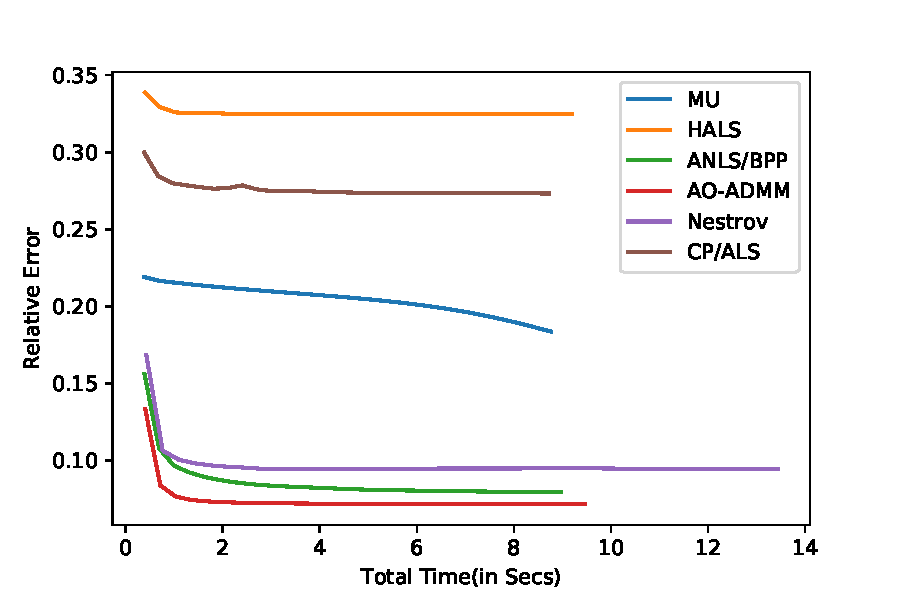
\includegraphics[width=0.45\textwidth, height=2in]{data/plots/accuracymouse96.pdf}
	}
	\caption{Relative error comparison of \MU, \HALS, \BPP\, \ADMM, \Nestrov\ on 4D Realworld Low Rank Tensor of size $1040\times1392\times69\times25$ on 64 Titan Nodes as $8\times8\times1\times1$ Processor Grid.}
	\label{fig:convergencemouse}
\end{figure}

\begin{figure}
   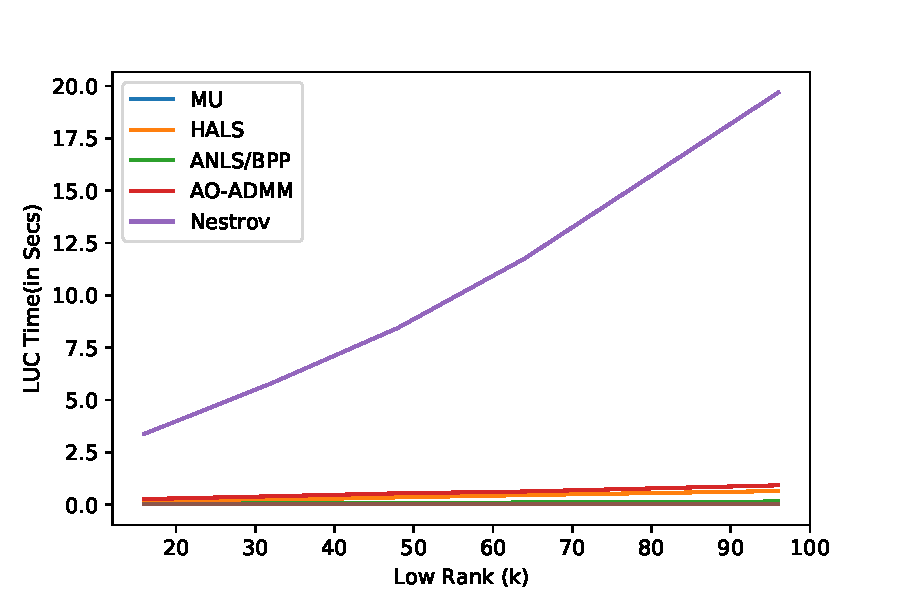
\includegraphics[width=0.45\textwidth, height=2in]{data/plots/lucmouse64.pdf}
	\caption{LUC comparison of \MU, \HALS, \BPP, \ADMM, \Nestrov\ on 4D Synthetic Low Rank Tensor of size $1040\times1392\times69\times25$ on 64 Titan nodes as $8\times8\times1\times1$ Processor Grid}
	\label{fig:luccompmouse}
\end{figure}

\begin{figure}
	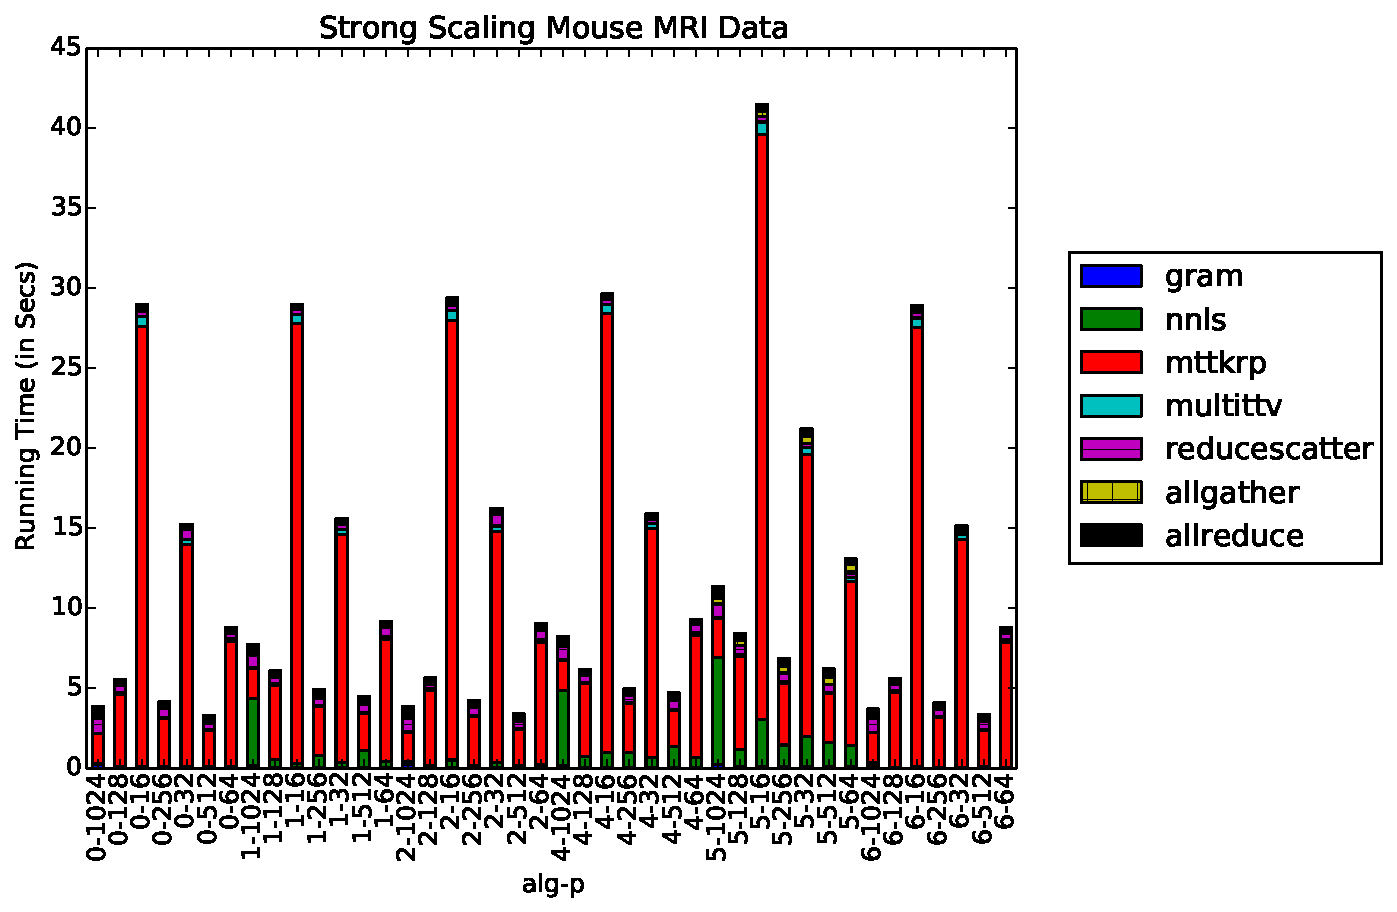
\includegraphics[width=\textwidth, height=3in]{data/plots/ssrw_mouse.pdf}
	\caption {Strong Scaling on Realworld Mouse MRI Dataset on 32, 64, 128, 256, 512 and 1024 nodes in Titan. The algorithms alg=0,1,2,4,5,6 are \MU, \HALS, \BPP, \ADMM, \Nestrov, \CPALS\ respectively.}
	\label{fig:synstrongscaling}
\end{figure}

